\documentclass{beamer}
\usepackage{amsmath}
\usepackage[english, russian]{babel}
\usepackage{bbm}
\usepackage{graphicx}
\usepackage[T2A, T1]{fontenc}
\usepackage[utf8]{inputenc}
\usepackage{tikz}
\usepackage{wrapfig}

\usetikzlibrary{shapes,arrows}
\tikzstyle{block} = [rectangle, draw,% fill=blue!20, 
    text width=10em, text centered, rounded corners]%, minimum height=4em]
\tikzstyle{line} = [draw, -latex']

\mode<presentation>
\usetheme{Warsaw}

\bibliographystyle{unsrt}


\title{Краевые моды и связанные состояния в топологических изоляторах}
\author[Е. Аникин]{Евгений Аникин \\
	научный руководитель\\
	чл.-к.~РАН~д.~ф--м.~н.~П.И. Арсеев}
\institute{ФИАН им. Лебедева}
\date{}

\begin{document}

\begin{frame}
    \titlepage
\end{frame}

\begin{frame}
    \frametitle{Двумерный топологический изолятор на основе HgTe}
    \begin{columns}[T]
        \begin{column}{0.5\textwidth}
            \begin{figure}[h]
                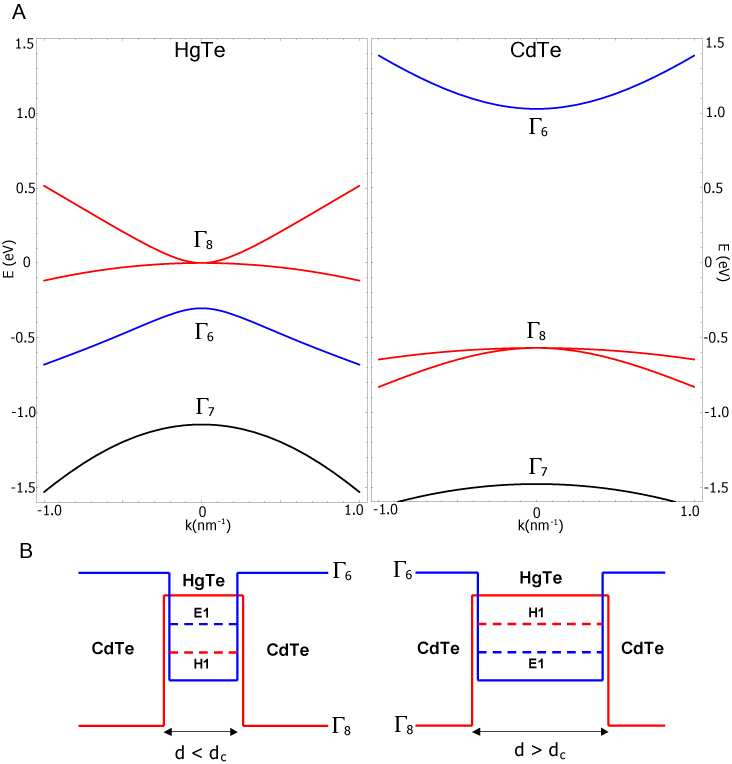
\includegraphics[width=0.95\linewidth]{quantum_well.png}
                \caption{Объемный спектр HgTe и CdTe и 
                         схематическое изображение квантовой ямы}
            \end{figure}
        \end{column}
        \begin{column}{0.5\textwidth}
            В квантовой яме образуются уровни размерного квантования. При
            $d < d_c$ спектр ямы нормальный, при $d > d_c$ --- 
            инвертированный.
        \end{column}
    \end{columns}
\end{frame}

\begin{frame}
    \frametitle{Гамильтониан Кейна}
    \begin{equation}
        H = \begin{pmatrix}
                    E_c + \frac{\hbar^2 k^2}{2m_s}E_{2\times 2} & T \\
                    T^\dagger & E_v + H_{L}
            \end{pmatrix}
    \end{equation}
    \begin{multline*}
        H_L = -\frac{\hbar^2}{2m_0}\left[
                \left(\gamma_1 + \frac{5}{2}\gamma_2\right)k^2 -
                2\gamma_2(\vec{k} \cdot \vec{J})^2 - \right. \\
                - \left.2(\gamma_3 - \gamma_2)(\{J_x J_y\} + \{J_x J_z\} + \{J_y J_z\})
                \vphantom{\frac{1}{2}}\right]
    \end{multline*}
    \begin{equation*}
        T = P\begin{pmatrix}
               -\frac{1}{\sqrt{2}}k_{+} & \sqrt{\frac{2}{3}}k_z  
                        & \frac{1}{\sqrt{6}} k_{-} & 0 \\
                0 & -\frac{1}{\sqrt{6}} k_{+} 
                        & \sqrt{\frac{2}{3}}k_z & \frac{1}{\sqrt{2}} k_{-} 
             \end{pmatrix}
    \end{equation*}
\end{frame}

\begin{frame}
    \frametitle{Эффективный гамильтониан для уровней размерного квантования}
        Эффективный гамильтониан для E1, H1 подуровней квантовой ямы HgTe:
        \begin{equation}
           \label{eff_so_ham}
            \scalebox{0.6}{%
            $
            H = \left(\begin{matrix}
                    \xi + \frac{1}{m}(2 - \cos{p_x} - \cos{p_y}) & 
                            2t(\sin{p_x} - i\sin{p_y})   \\
                    2t(\sin{p_x} + i\sin{p_y}) & 
                           - \xi - \frac{1}{m}(2 - \cos{p_x} - \cos{p_y}) \\
                \end{matrix}\right)
            $
            }
        \end{equation}
        Описывает топологический изолятор при $\xi < 0$
\end{frame}

\begin{frame}
    \frametitle{Краевые моды}
    \begin{columns}[T]
        \begin{column}{0.5\textwidth}
            \begin{figure}[h]
                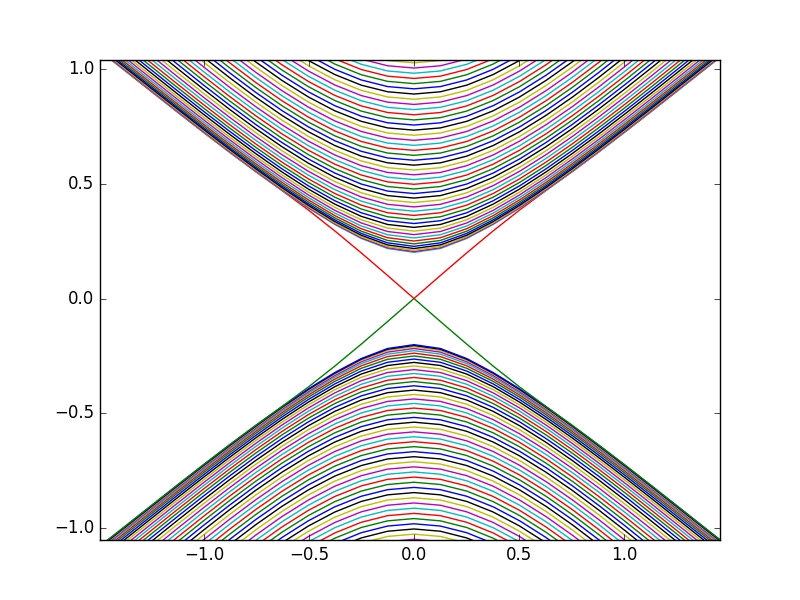
\includegraphics[width=0.95\linewidth]{edge_states.png}
                \caption{Спектр полосы ТИ: результат численной диагонализации}
            \end{figure}
        \end{column}
        \begin{column}{0.5\textwidth}
            На границе топологического изолятора образуются моды, пересекающие щель.
            Их закон дисперсии --- $\epsilon \approx \pm vk$ для двух проекций спина. 
            $T$--инвариантное возмущение не может привести к рассеянию краевых 
            электронов назад.
    
            Какие могут быть механизмы для рассеяния?
        \end{column}
    \end{columns}
\end{frame}

\begin{frame}
    \frametitle{Огибание препятствий}
    
\end{frame}
\end{document}
